\section{Implementation: Integer Linear Programming}
\label{sec:ILP}

Our matrix formulation above leads to the natural question: can we formulate loss function computation as a linear program?
Indeed, we will show that both the objective function and constraints
of the loss function optimization problem can be expressed as linear relationships.
By \cref{thm:LossEquivMatrices}, evaluating the loss function reduces to finding the maximum entries across a collection of matrix products listed in \cref{tab:theList}. The key idea is to treat the entries of all $M_\phi$ and $M_\psi$ matrices as variables and then solve a linear program that selects these entries so as to minimize the resulting loss.
However, due to the discrete nature of the problem, the resulting formulation takes the form of an integer linear program (ILP). 
This comes with a downside in complexity, as solving an ILP is NP-complete~\cite[Pg.~245]{Garey1979}.
That said, computing the interleaving distance is known to be NP-hard (see \cite{bjerkevik2017computational,bjerkevik2020computing}, and the discussion in \cref{sec:Problems}), so we have no reason to attempt to design an algorithm that runs in polynomial time. 
Nevertheless, developing efficient ILP solvers is an active area of research, resulting in many solvers that are extremely efficient in practice, so this translation allows us to take advantage of the current best known solvers. 

\subsection{ILP Model Description}
\label{ssec:ILP_model_description}
%
The goal of this optimization is either to find an $n$-interleaving (\cref{prob:BinaryDecision}) or search over possible $n$-assignments   to minimize the loss function (\cref{prob:LossComputation}).
This ends up being essentially the same setup, depending on whether we use the multiplication by distance matrices $D_\bullet^\bullet$ in \cref{tab:theList}. 
To that end, we describe the ILP here for the loss function version, since determining if there is an interleaving in (\cref{prob:BinaryDecision}) is the same setup but without inclusion of the $D$ matrices. 

In the case of finding the loss, the objective function for the ILP is to minimize $L_B(\varphi, \psi)$ over all possible $n$-assignments $(\phi,\psi)$. 
We denote the objective function as $\ell$ in the ILP.
As the loss is calculated on assignments, the entries in the blocks of the eight assignment matrices 
$M_\eta^A$ for $\eta \in \{ \phi, \phi^n, \psi, \psi^n\}$ and $A \in \{V, E\}$ serve as decision variables.
Using \cref{thm:LossEquivMatrices}, we know that the loss for each individual diagram can be computed by finding the maximum absolute value or the maximum of the ceiling of half the value among the entries of matrix multiplication terms listed in \cref{tab:theList}. 
Thus, we impose constraints in the ILP to connect the matrix representation of each term in $L_B(\varphi, \psi)$. 
We model the loss $\ell$ to be greater than or equal to the relevant entry in these matrices. 
Since it is a minimization problem, the ILP seeks the smallest $\ell$ that satisfies this condition, ensuring the equality.
Below we describe how the three diagram types (see \cref{tab:theList}) contribute to the ILP formulation. 
%

Reiterating above, our goal is 
\begin{equation*}
    \text{Minimize} \quad \ell 
\end{equation*}
with respect to the variables $ \{ x_{ij}^{\eta, A} \in M_\eta^A \mid  \eta \in \{ \phi, \phi^n, \psi, \psi^n\}, A \in \{V, E\} \}$ restricted to those entries in the blocks of the relevant matrices (we can implicitly assume $ x_{ij}^{\eta, A} = 0$ outside of these blocks). 
To ensure that the resulting matrices have a single one in each column, we include the first collection of constraints,
   \begin{align*}
        \text{Subject to}
        \qquad 
        \sum_i x_{ij}^{\eta,A} = 1 \qquad \forall x_{ij}^{\eta,A} \in M_\eta^A, \, \eta \in \{ \phi, \phi^n, \psi, \psi^n\}, \, A \in \{V,E\},
    \end{align*}
which ensure that all columns sum to 1. 


%
%
%
%
%
%
%
%
%
%
%
%
%
%
%
%
%
%



%
%

%
The next set of constraints are associated to  the edge-vertex parallelograms, where the corresponding diagrams are $\Lpl^{S_\tau, S_\sigma}$ and $\Lpr^{S_\tau, S_\sigma}$.  
For example, in the diagram $\Lpl^{S_\tau, S_\sigma}$, the loss is given by 
    %
    $
       \Lpl^{S_\tau, S_\sigma} =  \max \left( D_{G^n}^V \left(M_{\phi}^V \cdot B_F^{\uparrow} - B_{G^n}^{\uparrow} \cdot M_{\phi}^E\right)\right).
       $
    %
Therefore, we set the constraint that the objective function $\ell$ must be larger than any entry in the multiplied matrix. 
Thus, we include the constraints 
\begin{align*}
\text{Subject to} \quad 
%
 & \ell \geq  \max\left({D_{G^n}^V \left(M_{\phi}^V \cdot B_F^{\uparrow} - B_{G^n}^{\uparrow} \cdot M_{\phi}^E\right)}\right) \\
& \ell \geq \max\left({D_{G^n}^V \left(M_{\phi}^V \cdot B_F^{\downarrow} - B_{G^n}^{\downarrow} \cdot M_{\phi}^E\right)}\right)  \\
& \ell \geq \max\left({D_{F^n}^V \left(M_{\psi}^V \cdot B_G^{\uparrow} - B_{F^n}^{\uparrow} \cdot M_{\psi}^E\right)}\right) \\
& \ell \geq \max\left({ D_{F^n}^V \left(M_{\psi}^V \cdot B_G^{\downarrow} - B_{F^n}^{\downarrow} \cdot M_{\psi}^E\right)}\right).
%
\end{align*}
    We note that the $D$ and $B$ matrices  are constants in the ILP.
    Therefore, the matrix multiplication expression is linear and suitable for ILP.



For the thickening parallelograms, the corresponding losses are $\Lpl^{S_\rho, S_\rho^n}$ and $\Lpr^{S_\rho, S_\rho^n}$.  
As in the vertex edge case, we need to ensure that all entries in the relevant multiplied matrices from \cref{tab:theList} are bounded by $\ell$. 
Thus we add the following constraints 
\begin{align*}
\text{Subject to} \quad 
& \ell \geq \max\left( D_{G^n}^V \left(M_{\phi^n}^V \cdot I_F^V - I_{G^n}^V \cdot M_{\phi}^V\right)\right) \\
&\ell \geq \max\left( D_{G^n}^E \left(M_{\phi^n}^E \cdot I_F^E - I_{G^n}^E \cdot M_{\phi}^E\right)\right)\\ 
&\ell \geq \max\left( D_{F^n}^V \left(M_{\psi^n}^V \cdot I_G^V - I_{F^n}^V \cdot M_{\psi}^V\right)\right)\\
&\ell \geq \max\left( D_{F^n}^E \left(M_{\psi^n}^E \cdot I_G^E - I_{F^n}^E \cdot M_{\psi}^E\right)\right)
\end{align*}
    Similar to the edge-vertex parallelograms, the $D$ and $I$ matrices are constants in ILP, which makes these constraints linear.

    

Finally, we include constraints to control the entries on the triangle diagram matrices with corresponding loss functions  $\Ltd^{S_\rho}$ and $\Ltu^{S_\rho}$.   
We first  discuss the diagram $\Ltd^{S_{\sigma_i}}$ which operates on vertices. 
The loss contribution from this type of diagram can be obtained by finding 
    %
    $
    \max_{i} \Ltd^{S_{\sigma_{i}}} = \max \left\{ \left\lceil\tfrac{x}{2}\right\rceil  \, \middle|\,  x \in D_{F^{2n}}^V \left(I_{F^n}^V \cdot I_F^V - M_{\psi^n}^V\cdot M_{\phi}^V \right) \right\}.
    $
    %
Unlike the previous two types of diagrams, the expression $D_{F^{2n}}^V \left(I_{F^n}^V \cdot I_F^V - M_{\psi^n}^V\cdot M_{\phi}^V \right)$ is quadratic rather than linear, as it includes the term $M_{\psi^n}^V\cdot M_{\phi}^V$, which is a multiplication of two variable matrices. 
However, we can linearize the problem by introducing a collection of integer and binary reparametrization variables and adding them to the constraints.
    Furthermore, the ceiling function that we need to compute here is not a linear function either.
    This is taken care of with another reparametrization integer variable.
Specifically, we create the variables $\{z_{ijk}  \}$, one to represent each entry $x_{ij}^{\psi_n,V} x_{jk}^{\phi,V}$, so that if we construct the matrix $M$ where $M_{ik} = \sum_j z_{ijk} $, then 
${M = (M_{\psi^n}^V)_{ij}(M_{\phi^n}^V)_{jk}}$. 
Then, we get the following constraints for $\Ltd^{S_{\sigma_{i}}}$:
    \begin{align*}
        \text{Subject to} 
        \begin{alignedat}[t]{3}
        %
        \quad & 2c_{ij} \geq k_{ij} \quad  
            &\forall \quad k_{ij} \in D_{F^{2n}}^V \left(I_{F^n}^V \cdot I_F^V - M \right)\\
        %
        \quad & z_{ijk} \leq x_{ij}^{\psi^n,V} 
            &\forall \quad x_{ij}^{\psi^n,V} \in M_{\psi^n}^V\\
        \quad & z_{ijk} \leq x_{jk}^{\phi,V} \quad 
            &\forall \quad x_{jk}^{\phi,V} \in M_{\phi}^V\\
        \quad & z_{ijk} \geq x_{ij}^{\psi^n,V} + x_{jk}^{\phi,V} - 1\\
        \quad & \ell \geq c_{ij}.
        %
        \end{alignedat}
    \end{align*}
    %
    These constraints are only for one of the four relevant triangle diagrams, however the other setups are similar. 
    
%
Our full linear program is formulated to minimize $\ell$ subject to the constraints described above. Specifically, let
\[
V_{\max} = \max\{|V_H| \mid H \in F, F^n, G, G^n\}, \quad 
E_{\max} = \max\{|E_H| \mid H \in F, F^n, G, G^n\}.
\]
The total number of variables and constraints in the ILP can be bounded in terms of these graph sizes.

The primary binary decision variables are the entries of the eight assignment matrices $M_\eta^A$, where $A \in \{\varphi, \varphi^n, \psi, \psi^n\}$ and $A \in \{V, E\}$. Each matrix has a block structure, with one block for each function value $i \in [-L, L]$. Each block has size at most $V_{\max}^2$ (respectively $E_{\max}^2$) for vertex-type (respectively edge-type) matrices, yielding a total of $O\left(L \cdot (V_{\max}^2 + E_{\max}^2)\right)$ primary binary variables.

The remaining variables are auxiliary reparameterization variables $z_{ijk}$, introduced to linearize products such as $M_{\psi^n}^V M_\varphi^V$ appearing in the triangle-diagram constraints, along with integer variables $c_{ij}$ to handle ceiling operations. Each triangle product at level $i$ introduces one binary variable $z_{ijk}$ for each triple $(i,j,k)$, contributing up to $V_{\max}^3$ variables per function value. Across all four triangle diagrams, this yields $O\left(L \cdot (V_{\max}^3 + E_{\max}^3)\right)$ auxiliary variables.
%
Consequently, the total number of variables and constraints in the ILP is $O\left(L \cdot (V_{\max}^3 + E_{\max}^3)\right)$, which is polynomial in the input size. We note that the cubic dependence on $V_{\max}$ and $E_{\max}$ may be reducible with a more refined parameterization, which we leave for future work.
    
    
    
    


%

\subsection{Python Implementation Details}
\label{ssec:PythonImplementationILP}
    We implement the ILP using PuLP library in Python which is an open-source software package in Python specializing in modeling and solving mixed-integer linear programming problems \cite{mitchell2011pulp}. 
    Specifically, PuLP is equipped to solve ILP problems involving integer and binary variables, as in our case. 
    PuLP also integrates seamlessly with popular ILP solvers, both commercial (e.g. Gurobi \cite{gurobi}) and open source (e.g. CBC \cite{cbc}, GLPK \cite{glpk}), without having to alter the model formulation. 
    It is important to note that PuLP is exclusively designed to model \textit{linear} optimization problems, hence the extra work done in \cref{ssec:ILP_model_description} to linearize our ILP.    
    We choose PuLP over available non-linear modeling frameworks like Pyomo~\cite{hart2009python} because it is lightweight and has a simpler syntax, making it easier to interpret and update.
    Further, the design of PuLP is streamlined for ILP computation, reducing the computational overhead.
    We note that given an ILP, PuLP will return one of five options\footnote{This is discussed in the PuLP documentation at \href{https://coin-or.github.io/pulp/technical/constants.html}{coin-or.github.io/pulp/technical/constants.html}}: 
\textbf{(1) or (-1):} it terminates with the optimal solution (feasible or infeasible); 
\textbf{(0):} it cannot solve the problem given the time and memory constraints; 
\textbf{(-2):} the problem is unbounded; or 
\textbf{(-3):} the problem is undefined.
However, in our experiments, the solver always terminates successfully (output \textbf{(1)} or \textbf{(-1)}). 

    \begin{figure}
        \centering
        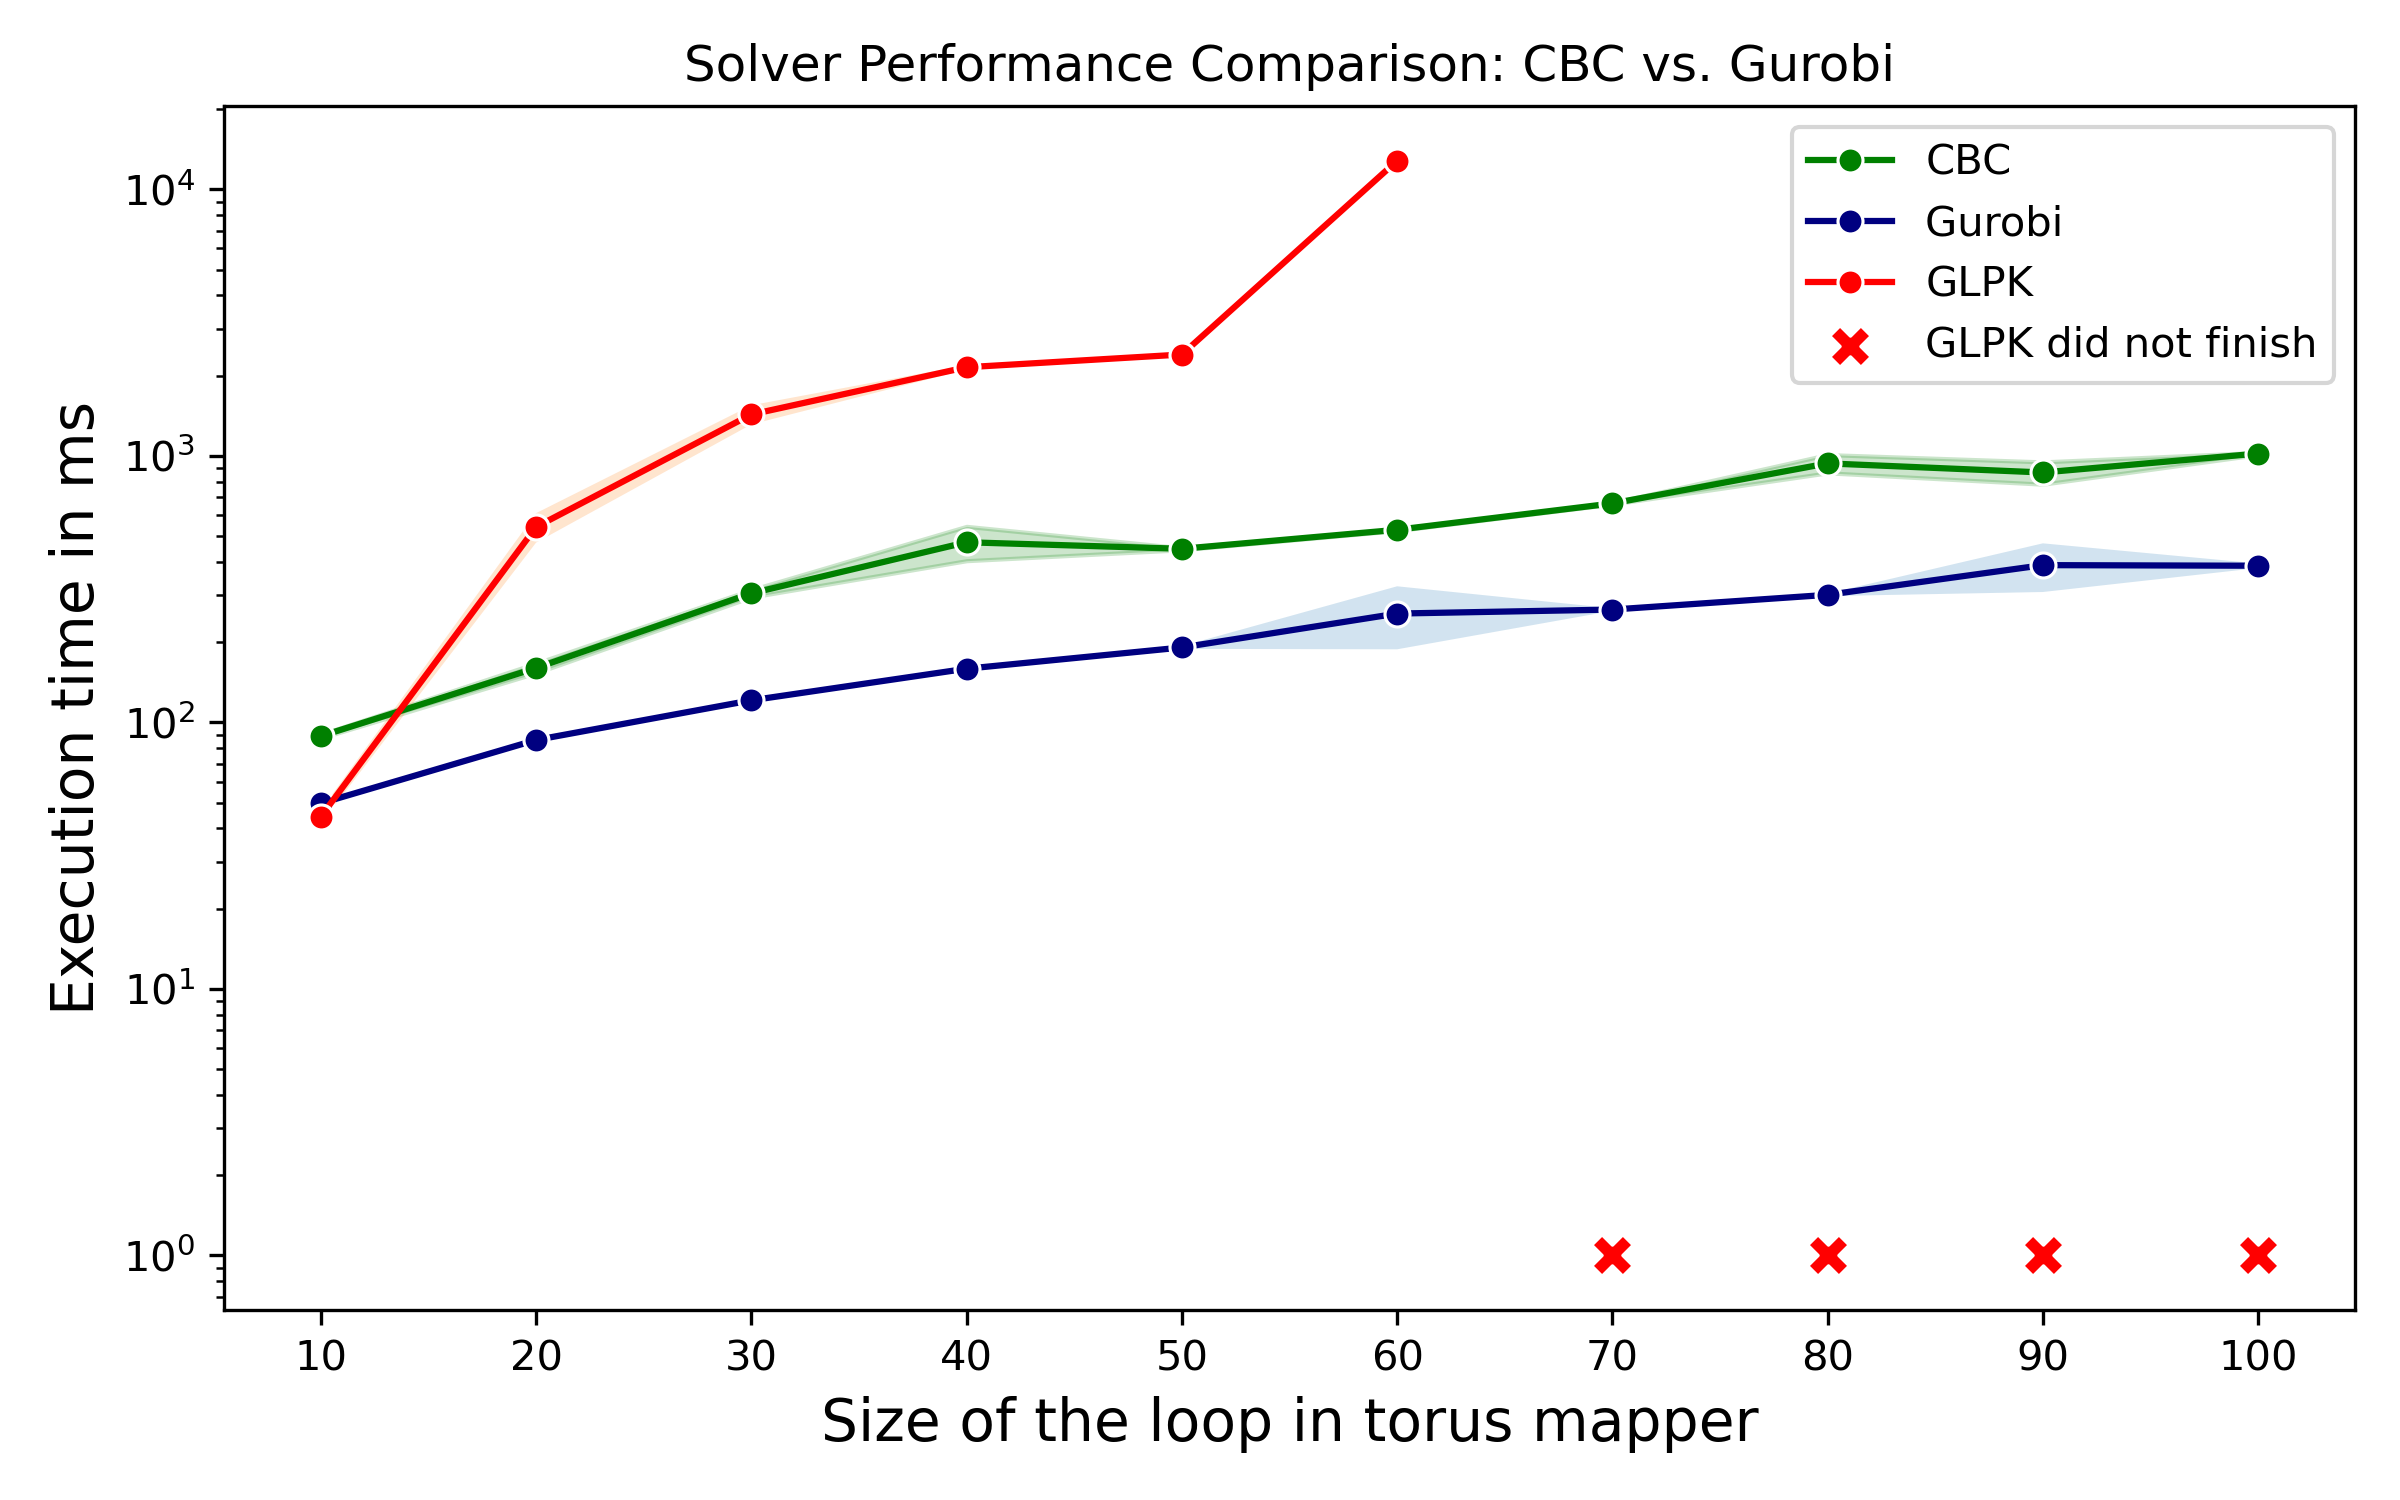
\includegraphics[width=0.7\linewidth]{figures/solver_timing.png}
        \caption{Time taken by different solvers to optimize the loss for the torus and line mappers.}
        \label{fig:solver_timing}
    \end{figure}
    
    We test our ILP implementation with simple input examples to make a choice of solver for use in PuLP; 
    the specifics of this particular example pair will be given in \cref{ssec:line_torus_sec}.
    In this example, increasing loop size increases the size of the input graphs, thus the size of the ILP increases.
   We test two open-source solvers, CBC (COIN-OR Branch and Cut) and GLPK (GNU Linear Programming Kit), as well as the commercial solver Gurobi. 
    %
    The results are shown in \cref{fig:solver_timing}.
    We see that for smaller problem size (up to a loop size of 20 in the torus mapper), all of the solvers take less than one second to optimize the loss.
    However, as the size of the loop increases, the GLPK solver becomes significantly slower than CBC or Gurobi. 
    %
    In fact, for loop sizes of 70 and above, GLPK fails to complete computation even after 15 minutes of runtime.
    As expected, the commercial solver Gurobi is highly optimized, resulting in superior performance. 
    Both CBC and Gurobi's computation times increased approximately linearly with the loop size.    
    Among the open-source solvers we tested, CBC is slower than Gurobi but is still able to optimize large problems effectively.
    Since CBC is the default solver in PuLP, it is also more accessible from a user’s perspective.
    Thus, for the rest of the experimental section, we exclusively use the CBC solver inside of PuLP.
    The code for our implementation is available in the Python package \texttt{ceREEBerus} \cite{cereeberus}.
    %
    %
    
    
       
%


%
%
%
%
%
%
%
%
%
%
%
%
%





 



 %
 %
 %
 %
 %
 %
 %
 %
 %
 %
 %
 %
 %
 %
 %
 %
 %
 %
 %
 %
 %
 %
 %
%
%
%
%
%
%
%
%
%
%
%
%
%
%
%
%
%
%
%
%
%
%
     
 %
    







%
%

%
%
%
%
%
%
%
%
%
%
%

%
%



